\section{Introduction} \label{sec:intro}

%P1: SMR difinition; traditional network message passing; reliable; attractive
% for general servers. Agree-execute: must reach consensus and then execute a
% request. Emphasis ordering services, Scatter, 8~12 nodes.

\paxos~\cite{paxos:practical,paxos,paxos:simple,paxos:complex}) plays a core
role in datacenters and distributed systems, including ordering
services~\cite{ellis:thesis,manos:hotdep10,scatter:sosp11},
leader election~\cite{zookeeper, chubby:osdi}, and
fault-tolerance~\cite{eve:osdi12,rex:eurosys14,crane:sosp15}. A \paxos service
runs the same program on a group of replicas and enforces a strongly
consistent order of inputs for this program, as long as a quorum (typically,
majority) of replicas still behave correctly.

% TBD: Scatter description is not very clear; on replica sub key range part.
Due to this strong fault-tolerance, \paxos is widely served in many systems.
For instance, Scatter~\cite{scatter:sosp11} runs 8$\sim$12 replicas in each
\paxos group to order client requests, and it lets replicas respond requests
in parallel. A bigger group size will improve Scatter throughput. Moreover, 
recent state machine replication (SMR) systems~\cite{ crane:sosp15,
eve:osdi12, rex:eurosys14} use \paxos to greatly improve the availability of
general server programs.




% Typically, \paxos assigns a replica as the leader to propose
% consensus requests, and the other replicas agree or reject requests.
% An input consensus can achieve as long as a majority of replicas
% agree, thus SMR can tolerate various faults such as minor replica failures.


% P2: Performance too slow. Agree first and then execute. Even three nodes, one
% round-trip (~400 us). Not for performance critical servers such as key-value.
% Batching: addressed throughput but not latency.
Unfortunately, despite these advances, the high \paxos consensus latency makes
many systems suffer. For efficiency, \paxos typically assigns one replica as
the leader to invoke consensus requests, and the other replicas as backups to
agree on requests. To agree on an input, at least one message round-trip is
required between the leader and a backup. A round-trip causes big latency as it
goes through TCP/IP layers such as software network stack and OS kernel. This
latency could be acceptable for leader elections~\cite{chubby:osdi,zookeeper} or
heavyweight transactions~\cite{crane:sosp15,eve:osdi12}, but undesirable for
key-value stores~\cite{redis,memcached}.
% To address this challenge,
% some systems~\cite{calvin:sigmod12,rex:eurosys14} batch requests into one
% consensus round. However, batching will only mitigate throughput lost and it
% will aggravate request latency.
% As a possible consequence, although many recent storage
% systems~\cite{drtm}
% explicitly stated that they needed a replication system for high availability,
% they finely didn't adopt the batching approach.

% P3: Another problem: scalability. As more nodes are in replica group, it is
% getting much more slower to reach quorum. Event-driven to increase
% parallilism, but still slow: despite the large latency, context switches (400
% us).

As replica group size grows, \paxos consensus latency increases
drastically~\cite{scatter:sosp11} due to the linearly increasing number of 
consensus messsages. To improve scalability,
one approach is introducing parallel techniques such as 
multithreading~\cite{zookeeper, spaxos} or asynchrous IO~\cite{crane:sosp15, 
libpaxos}. However, the high latency of TCP/IP round-trips still exist, and 
the synchronizations in these techniques
frequently involve expensive OS events such as context switches. We ran four
\paxos-like protocols~\cite{zookeeper, crane:sosp15, spaxos, libpaxos} on 40Gbps
network with only one client sending consensus requests, and we found that: when
replica group size increased from 3 to 9, the consensus latency of these
protocols increased by \tradlatencyincreaselow to \tradlatencyincreasehigh, and
\systemcostlow to \systemcosthigh of the increase was in OS kernel.

A second approach to scale \paxos is running multiple \paxos instances,
including partitioning program states~\cite{scatter:sosp11,dssmr,ssmr},
splitting consensus leadership~\cite{mencius:osdi08,spaxos}, and hieratical
replication~\cite{manos:hotdep10,scatter:sosp11}. However, the core of
these systems, \paxos, still
scales poorly~\cite{ellis:thesis,scatter:sosp11,manos:hotdep10}.

%  advanced
% replication
% models are proposed, including
% multi-leader~\cite{epaxos:sosp13,mencius:osdi08},
% cluster~\cite{manos:hotdep10}, and nested consensus
% models~\cite{scatter:sosp11}.

% One
% scalling approach (\eg, ~\cite{crane:sosp15}) may be using an event-driven
% model (\eg, Libevent~\cite{libevent}) to improve the parallilism of replicas'
% consensus round-trips. However, the high latency of a single round-trip still
% exists.
% and synchronization context switches (often takes hundreds of \us) in
% the event loop of this model also adds latency.


% The second challenge is that an automated, fine-grained approach is needed to
% avoid execution divergence of active (\ie, alive) replicas. Even in the absence
% of replica failures or network partitions, the executions of different replicas
% can still diverge due to contention of
% inter-thread resources~\cite{coredet:asplos10} (\eg, shared memory) and systems
% resources~\cite{racepro:sosp11} (\eg, files and network ports). This challenge
% not only lies in standard SMR systems which require deterministic executions,
% but it is also pervasive in commodity replication systems (\eg, \redis,
% \memcached, and \mysql) that seek for fault-tolerance in some degree.

% P4.0: opportunity, RDMA. We argue that, network layers are not inherent.
% Memory semantic.
Fortunately, Remote Direct Access Memory (RDMA) becomes a promising solution
as it becomes common in datacenters. RDMA not only bypasses the OS kernel,
but also provides dedicated, network hardware to achieve ultra fast round-trip.
For instance, the fastest RDMA operation allows a process to directly write to
a remote replica's process, without involing the remote OS kernel or CPU (\ie,
``one-sided" operations). As a common RDMA practice, to ensure a write
successfully resides in the remote memory, local process polls an ACK sent
from remote NIC. Such an RDMA round-trip takes only
$\sim$3 \us~\cite{pilaf:usenix14}.


% A strawman approach: DARE. RDMA communication primitives themselves have
% scalability issues.
% DARE weaken memory semantic. Need to come up with a reason.
However, due to the unrichness of RDMA primitives, fully exploiting RDMA
speed in software systems is widely
considered challenging~\cite{pilaf:usenix14,herd:sigcomm14,
farm:sosp15,dare:hpdc15}. For instance, DARE~\cite{dare:hpdc15} presents a
sole-leader, RDMA-based \paxos protocol, which lets the leader does all
RDMA workloads. This protocol was fast with three to five replica group.
However, our evaluation shows that, as replica group grows, the leader met
scalability bottlenecks (\eg, polling ACKs), and its consensus latency
increased by \darescalability as the group size increased by 35x
(\S\ref{sec:evaluation}).

% For
% instance, one-sided RDMA operations eliminate remote replicas' participations,
% but traditional \paxos protocols require non-leader replicas to examine the
% leader's consensus requests.

% First, the leader uses RDMA to write the consensus requests to all replicas and
% polls RDMA ACKs to check whether the writes succeed. Second, for the successful
% writes, the leader does another round of RDMA writes to mark the writes as
% successful on other replicas, and poll ACKs on these writes. One a majority of
% successful writes in the second round, DARE reaches a consensus.

% Our key idea: pure remote-memory consensus. A fully scalable RDMA Paxos
% should allow leader to process requests pure on memory. Leader and replica
% % join % consensus; have stable storage with this benefit.
% Why is this idea fast. Mulithreading.
% We: heavily exploiting memory semantic of RDMA. Use more CPUs; save ACKs.
Our main idea is that we should carefully separate RDMA workloads among
the leader and the backups, especially in such a latency- and scalability-
sensitive context. For instance, we should let both the leader and backups
do RDMA writes directly on the desination replicas' memory, and let all
replicas poll their own local memory. Although doing so may consume more CPU
resources than a sole-leader approach, it has two benefits. First, the
leader has less RDMA workloads. Second, both leader and backups can get rid of
the expensive RDMA ACK polling and they just receive consensus messages on their
local memory efficiently. An analogy is that threads receive other threads' data
via bare memory, a efficient and scalable computation pattern.


% An analogy is that threads receive other threads' data and
% signals via bare memory, a fast and scalable multithreading pattern. Now the
% only RDMA primitive our \paxos replicas involve is just sending RDMA writes
% (\ie, copying the data to be sent to NIC). Our evaluation showed that
% most of such outbound RDMA write operations took less than 0.2 \us, much faster
% faster than inbound RDMA operations.

% Why is this idea feasible. Paxos can already handle unreliability.
% Tech challenge? data integrity. Storage. Checkpoints? Others?
In deed, this idea raises reliability issues because now the leader has no clue
on whether the remote writes succeed. Fortunately, \paxos's protocol already
tolerates various reliability issues, including message losses caused by
hardware or program failures. Now one just needs a runtime system to efficiently
ensure the atomicity of remote writes among replicas (\S\ref{sec:normal}).



% As a common RDMA practice, to ensure that such a write
% successfully resides in the memory of a remote process, the local process
% should wait until the remote NIC (network interface card) sends an ACK to the
% local host's NIC. An evaluation~\cite{pilaf:usenix14} shows that such a write
% round-trip takes only $\sim$3 \us in the Infiniband networking
% architecture~\cite{infiniband}.

% However, it is technically challenging to fully exploit RDMA speed in \paxos
% protocols due to the unrichness of RDMA features. We present this challenge in
% detail by elaborating two possible approaches below. One straightforward
% approach is IP over Infiniband (IPoIB). This approach emulates TCP/IP on RDMA
% hardware so that traditional \paxos implementations can enjoy RDMA speedup
% without modifications. However, this loose combination of RDMA and \paxos is
% still one order of magnitude slower than fastest RDMA operations because IPoIB
% goes through the OS kernel and copies network data between kernel and user
% space.

% To the best of our knowledege, DARE's approach achieves the fastest consensus
% speed in existing approaches because all communications are simply replaced
% with the fatest RDMA writes (although we argue that a stable storage for
% consensus requests should be added to ensure \paxos durability).

% However, this
% approach faces a scalability challenge: to ensure a remote replica is alive,
% each step has to wait ACKs from the previous step before it starts, and each
% RDMA write has to wait for its own ACK. In this pure leader-based algorithm,
% ACKs are necessary for every next step to start. As the replica group size
% grows, the leader has to do RDMA writes to remote replicas one by one, making
% its consensus latency grows linearly to replica group size (confirmed in our
% evaluation).
%
% to address this scalability challenge is that
% simply replacing RDMA writes with \paxos communications is not sufficient, and
% In addition to mitigating consensus latency, RDMA creates
% new opportunity to address the \paxos scalability problem, because we
% can integrate RDMA features \emph{tightly} within the fault-tolerant nature of
% \paxos. In essence, \paxos already tolerates various faults, including
% machine failures and process crashes. Therefore, we can safely ignore the ACKs
% in RDMA writes and let \paxos handle the (un)reliability of these writes.
%
% This integration of \paxos and RDMA features looks simple, but it leads to
% a fast, scalable \paxos consensus algorithm with three steps. First, the leader
% stores a consensus request in local stable storage. Second, it does RDMA writes
% in parallel to put this request to the memory of remote replicas without
% waiting any RDMA ACKs. Remote replicas also work in parallel: they poll from
% their local memory, store this request in local storage, and send consensus
% replies to the leader with RDMA writes, without waiting any RDMA ACKs
% either. Third, once the leader sees a majority of replies in local memory,
% a consensus is reached.
%
% In the second step of this algorithm, both the leader and remote replicas work
% in parallel, thus a complete consensus latency approximately consists of
% three operations: a leader's write to stable storage, a remote replica's write
% to local storage, and a RDMA write round-trip. This consensus
% latency is no longer firmly correlated with replica group size (confirmed in
% our evaluation); its scalability is now mainly bounded by the capacity of
% outbound RDMA writes in the NIC hardware. By making the core of \paxos
% scalable, other advanced replication
% models~\cite{epaxos:sosp13,mencius:osdi08,scatter:sosp11,manos:hotdep10} can
% scale even better.
%  (currently, 16~\cite{herd:sigcomm})

% P4: Falcon; key features. Hook sockets in servers.
Leveraging this idea, we present \xxx,\footnote{We name our system after
falcon, one of the astest birds.} a new RDMA-based \paxos protocol and its
runtime system. In \xxx, all replicas directly write to desination
replicas' memory and poll messages from local memory, and our runtime system
other several technical challenges such as messsage atomiciy
(\S\ref{sec:normal}), efficient logging (\S\ref{sec:logging}), and failure
recovery (\S\ref{sec:checkpoint}).

Similar to general SMR systems~\cite{rex:eurosys14,crane:sosp15},
\xxx's design supports general, unmodified server programs: within \xxx, a
program just runs as is, and \xxx automatically deploys this program on replicas
of machines. It intercepts inputs from a server program's inbound socket calls
(\eg, \recv) and invokes our \paxos protocol to enforce same inputs
across replicas.



% \xxx then provides an optional
% rollback/restore mechanism to make an effort to restore the diverged replicas.
% Because hash computation is efficient and output consensus is invoked rarely,
% this output checking protocol introduced negligible performance impact in our
% evaluation.

% In a consensus protocol level, \xxx carefully tackles several technical
% challenges, including handling an atomicity challenge (\S\ref{sec:normal}) and
% concurrent connections (\S\ref{sec:concurrent}).

% If \xxx finds that
% a replica produces an different output from what other replicas agree on, \xxx
% recovers this replica to a previous program checkpoint and re-executes inputs
% that have been agreed on from the checkpoint.

% P6: Falcon: output checker.
% However, to practically replicate general server programs, only enforcing same
% inputs is often not enough. An automated, efficient output checking mechanism
% that can improve the assurance on ``replicas run in sync" is still missing in
% existing SMR
% systems~\cite{calvin:sigmod12,rex:eurosys14,crane:sosp15,dare:hpdc15}.
% Most server programs use multithreading to harness the power of multi-core
% hardware. Nondeterminism~\cite{racepro:sosp11,dmp:asplos09,coredet:asplos10,
% cui:tern:osdi10, kendo:asplos09,
% dthreads:sosp11,peregrine:sosp11,parrot:sosp13,determinator:osdi10} caused by
% contentions in inter-thread resources (\eg, global memory and locks) and systems
% resources (\eg, network ports) can easily cause program execution states to
% diverge across replicas and compute wrong outputs to clients.
%
% To tackle nondeterminism, SMR systems either use deterministic multithreading
% and replay approaches~\cite{rex:eurosys14,crane:sosp15,ddos:asplos13}, or they
% rely on manually annotating share states in program code to detect execution
% divergence~\cite{eve:osdi12}. These approaches fall short in performance
% or automation.



% This
% protocol automatically, efficiently checks the fine-grained network outputs
% and improves assurance on whether replicas run in sync.

% A practical
% output checking mechanism is missing in widely deployed replication
% systems (\eg, \redis and \mysql) either, although these replication sytems
% provide weaker fault-tolerance or consistency guarantees than SMR for better
% performance.
%
% Two approaches for checking whether replicas run in sync exists. Existing
% widely deployed systems typically use \v{ping} to check whether replicas run in
% sync, but this coarse-grained checking will miss output divergence caused by
% tricky concurrency bugs~\cite{lu:concurrency-bugs}. Eve

% First, introduce naive approach. IPoverIB.

% P5: Falcon: RDMA input coordination. Persistent stores; two RDMA writes
% between two machines; no context switch.
% To coordinate inputs among replicas, \xxx intercepts a server program's socket
% APIs (\eg, \recv) to caputure inputs and introduces a new RDMA-accelerated
% \paxos protocol to let replicas agree on these inputs. To ease understanding
% and checking tooks. this protocol complies with common style of popular paxos
% protocal~\cite{paxos:practical}. In the normal case of this protocol, contrast
% to existing implementations which require one network round-trip (\ie, two
% messages for every two replicas), our protocal only requires two most efficient
% one-sided write operations.

% P5.1: Support read-only optimization.



% To address this challenge, recent SMR systems leverage either deterministic
% multithreading techniques~\cite{rex:eurosys14,crane:sosp15} or detecting
% divergence of execution by manually annotating program states by threads,
% artificially trading off performance or automatacity.

% Typical commodity
% replication systems ignore this challenge and use `ping" to check whether
% replicas are working as expected, but this coarse-grained approach can not
% detect execution divergence of resource contentions because a program can just
% compute wrong outputs without crashing.

% Our key idea is that we don't need to a program's every (or every batch)
% network outputs because they most replicas's outputs indicate that this output
% is most likely the produced one. Either necessary or sufficient. Not necessary
% because most executions already produce same program behaviors (including
% outputs) even with concurrency bugs. Not sufficient because it could be all
% replicas producing the same buggy output and bypass consensus protocols. All we
% need is just lazily compare outputs and if a divergence is detected, we roll
% back programs and re-execute them.

% To implement this idea, \xxx's output verification protocol first . network
% outputs on each individual replica, computes  hash values incremental:
% compute the hash value of a union of last hash value and the output  and
% periodically invoke our \paxos consensus protocol to exchange the hash value.
% Then, if minor replicas' outputs diverge from the majority ones, we just roll
% back and re-execute these minor replicas without perturbing the others to agree
% on and process new inputs. If a majority can not reach, \xxx simply rolls back
% the XXX (leader?). Evaluation confirmed that XX.XX\% cases.


% P7: conceptual level: complete architecture. agree-execute-enforcement.
% In a conceptual level, to provide pratical SMR service for general programs,
% \xxx presents a new agree-execute-verify execution model, which contrasts from
% previous agree-execute models and execute-verify models. We argue that agree is
% essential to SMR due to its strong fault-tolerance on machine failures and
% packet losses (even RDMA networks have packet loss when machines fail or
% programs crash). Having a general input coordination protocol also mitigates
% the need of writing application-specific input mixer and manually code
% annotation. Moreover, a automatic, fast output verification protocol is
% essential to SMR because we aim to replicate general, diverse server programs
% that may diverge due to resource contentions. In sum, by coordinating inputs
% and verifying outputs among replicas, \xxx practically enforces same execution
% states and outputs among replicas.

% P8: implementation. POSIX. support checkpoint.
We implemented \xxx in Linux. \xxx intercepts POSIX inbound socket calls
(\eg, \accept and \recv) to coordinate inputs using the Infiniband
RDMA architecture. To improve the assurance that replicas run in sync, on top
of \xxx's \paxos protocol, it also provides an efficient network output
checking protocol, a practical feature that may promote \xxx's deployments. To
recover or add new replicas, \xxx leverages \criu~\cite{criu} to periodically a
program on one backup, so it does not affect other replicas to reach consensus
efficiently.

% P9: Evaluatuion, with highlight items, match abstract, but more details.
We compared \xxx with five popular, open source \paxos-like implementations,
including four traditional ones (\libpaxos~\cite{libpaxos},
\zookeeper~\cite{zookeeper}, \crane~\cite{crane:sosp15} and
\spaxos~\cite{spaxos}) and a RDMA-based one (\dare~\cite{dare:hpdc15}). \spaxos
is designed to achieve scalable throughput when more replicas are added. We
also evaluated \xxx on \nprog widely used or studied server programs, including
\nkvprog key-value stores (\redis~\cite{redis}, \memcached~\cite{memcached},
\ssdb~\cite{ssdb}, and \mongodb~\cite{mongodb}), one SQL server
\mysql~\cite{mysql}, one anti-virus server \clamav~\cite{clamav}, one multimedia
storage server \mediatomb~\cite{mediatomb}, one LDAP server
\openldap~\cite{openldap}, and one advanced transactional database
\calvin~\cite{calvin:sigmod12} (with \zookeeper~\cite{zookeeper} as its SMR
protocol). Our evaluation shows that

\begin{tightenum}
\item \xxx achieves both one order of magnitude better scalability and one
order of magnitude faster consensus latency than literature.
Figure~\ref{fig:summary} shows a summary. \xxx's consensus latency was faster
than four popular \paxos implimentations by \comptradlow to \comptradhigh on
three to nine replicas. \xxx is faster than \dare by \fasterDARElow to
\fasterDARE. When increasing the replica group size from three to 105 (a 35x
increase), \xxx's consensus latency increases merely from \xxxlatencythree to
\xxxlatencyonezerofive (a \xxxscalability, sub-linear increase).

\item \xxx is general. For all \nprog evaluated programs, \xxx ran them without
any modification except \calvin (we added a \nlinescalvin-line patch to make
\calvin's client and server communicate with sockets).

\item \xxx incurs low overhead on \nprog widely used server programs.
With nine replicas, compared to servers' own unreplicated executions, \xxx
incurred merely \tputoverhead overhead on throughput and \latencyoverhead on
response time in average.

% \item \xxx is robust. On \paxos leader failures, \xxx's leader election
% latency was reasonable and scalable.

% \xxx's consensus latency is \fasterthanzookeeper
% faster than \calvin's SMR service \zookeeper.





% \item \xxx is extensible. To extend optimization on read-only requests, XX
% lines of code in our two provided APIs, \xxx is able to avoid the read-only
% requests in \redis to do consensus and XX times faster than \redis's own
% replication system.

\end{tightenum}
% % tighten items, highlighted.

% P10: Conceptual contribution. Applications: other replications, parallel
% program % analysis, and datacenter OS (it's efficiency and strong consistency
% makes % system calls go beyond single machine).
% New design space. comprehensive model. many applications: other replications,
% parallel analysis, datacenter OS.
Our major contribution is the idea of pure remote-memory consensus. This simple
yet effective idea leads to \xxx, a fast, scalable \paxos runtime system. \xxx
has the potential to largely improve the scale and speed of existing \paxos
services~\cite{scatter:sosp11,manos:hotdep10,crane:sosp15,rex:eurosys14}. For
instance, Scatter~\cite{scatter:sosp11} previously deployed 8 to 12 replicas in
each \paxos group, now it can deploy one order of magnitude more replicas in
each group with much faster consensus latency. Moreover, a general and
deployable service, \xxx may largely promote the deployments of \paxos and
improve the consistency and fault-tolerance of various systems in datacenters.

% \xxx
% can also be applied to broad areas, including other replication protocols (\eg,
% byzantine fault-tolerance~\cite{zyzzyva:sosp07,pbft:osdi99}), distributed
% program analyses, and future datacenter operating systems (\S\ref{sec:apps}).
% All \xxx source code, benchmarks, and evaluation results are
% available at \github.
% In addition, a fast, general SMR service has been long persued as a fundamental
% building block for the emerging datacenter operation system.

% P10: Engineering contribution. Potential to substitue customized replication
% in commodity systems and use a general ones. Easy to verify, easy to get
% right, easy to use.
% Our major engineering contribution includes the \xxx implemention and its
% evaluation on \nprog diverse, widely used server programs. Due to the lack of a
% general SMR system, industrial developers have spent tremondous efforts on
% building specific replication systems for their own programs and ``invent the
% wheels again and again". Note that understanding, building, and maintaining a
% usable SMR systems requires extreme expert knowledege, burdens, and are
% extremely challenging (so many \paxos papers). For example, the \redis or
% \memcached lag bug. Our \xxx system and evaluation has shown promising results
% on building a fast, general, and extendible SMR system and help developers
% greatly release these burdens. We have released all \xxx's source code,
% benchmarks, and raw evaluation results at \github.

% P11: Remaining of paper.
The remaining of this paper is organized as follows.
\S\ref{sec:background} introduces background on \paxos and RDMA features.
\S\ref{sec:overview} gives an overview of our \xxx system. \S\ref{sec:input}
presents \xxx's consensus protocol and its runtime system. \S\ref{sec:output}
describes the output checking protocol. \S\ref{sec:discuss} compares \dare with
\xxx, and discusses \xxx's current limitations and applications in other areas.
\S\ref{sec:evaluation} presents evaluation results, \S\ref{sec:related}
discusses related work, and \S\ref{sec:conclusion} concludes.

\begin{figure}[t]
\centering
\vspace{-.10in}
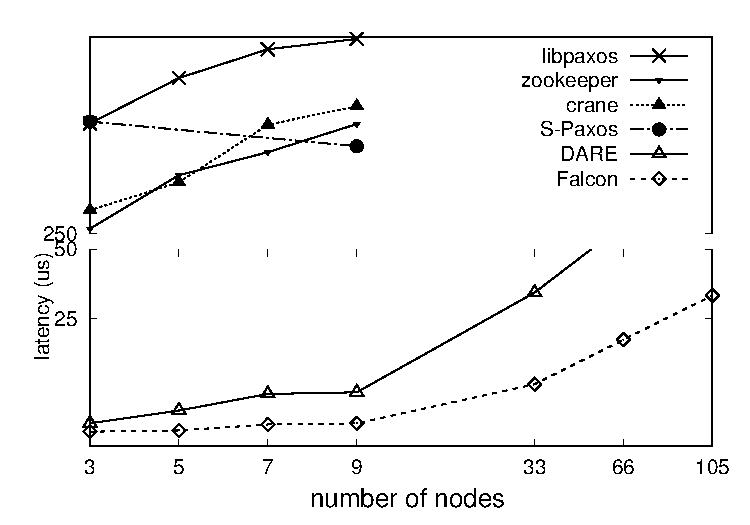
\includegraphics[width=.45\textwidth]{figures/traditional_paxos_latency}
\vspace{-.15in}
\caption{{\em Consensu latency of six \paxos-like protocols.}}
\label{fig:scalability}
\vspace{-.20in}
\end{figure}
